\section{Exercise 4}
\subsection*{4.1}
When we are working with images with a background which gradually changes intensity, i.e. when some of the background is light, and some of the background is dark, it can be hard for intensity based segmentation approaches to segment correctly. However, an edge based approach would perform well. An example would be \autoref{ex1} (first image taken from segmentation lecture slides).\\
Intensity based approaches are also problematic when we are segmenting blurred images, as the edges becomes gradually 'sharp' and thus, a small change in the threshold might result in a big difference in the size of the segmented object. Also what previously was right angles now becomes more soft. An example of this can be seen in the images from the segmentation lecture slides in \autoref{ex2}.\\
A more broad issue is the consistency of intensity based approaches, as the lighting of the scene might brighten or darken the image (this can both be uniformly and non-uniformly). That is, if we develop an automatic pipeline of image processing where we process several images of the same scene, but with different lighting, we can not expect the same amount of quality in the segmentation. This could be a big issue in a self driving car which should be able to drive during both day and night.

\begin{figure}[H]
	\centering
	\begin{subfigure}[b]{0.45\linewidth}
		\centering
		
\includegraphics[width=0.8\linewidth]{Materials/E4/background}
		\caption{Image with gradually changing background.\\\hfill}
	\end{subfigure}
	\hfill
	\begin{subfigure}[b]{0.45\linewidth}
		\centering
		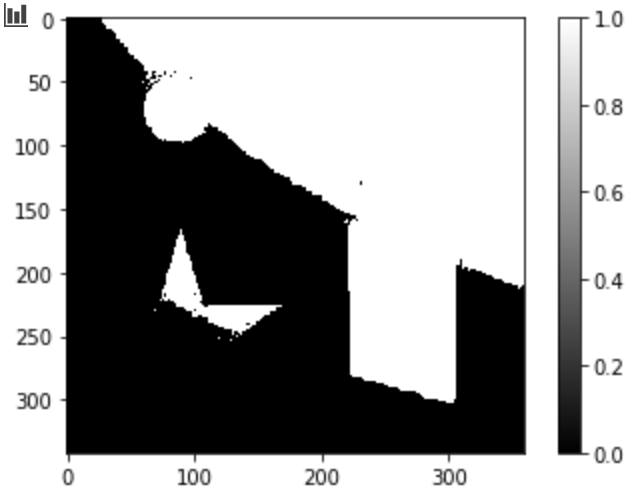
\includegraphics[width=\linewidth]{Materials/E4/intens_seg_res}
		\caption{Intensity based segmentation approach. Threshold at 75.}
	\end{subfigure}
	\\
	\begin{subfigure}[b]{0.45\linewidth}
		\centering
		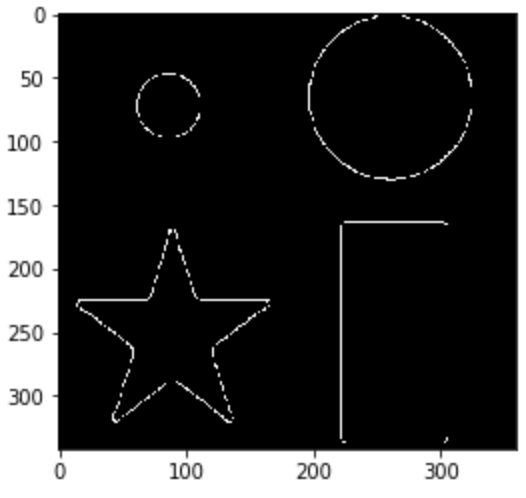
\includegraphics[width=\linewidth]{Materials/E4/canny_seg_res}
		\caption{Canny edge detection. $\sigma = 3$, low threshold = 0 and high threshold = 10.}
	\end{subfigure}
	\caption{Example 1 of problems with intensity based segmentation.}
	\label{ex1}
\end{figure}

\begin{figure}[H]
	\centering
	\begin{subfigure}[b]{0.35\linewidth}
		\centering
		
\includegraphics[width=\linewidth]{Materials/E4/ex2sharp}
		\caption{Sharp example image.}
	\end{subfigure}
	\hspace{1.5cm}
	\begin{subfigure}[b]{0.35\linewidth}
		\centering
		
\includegraphics[width=\linewidth]{Materials/E4/ex2blurred}
		\caption{Blurred example image.}
	\end{subfigure}
	\\
	\begin{subfigure}[b]{0.35\linewidth}
		\centering
		
\includegraphics[width=\linewidth]{Materials/E4/ex2soft}
		\caption{Example image after intensity based segmentation.}
	\end{subfigure}
	\caption{Example 2 of problems with intensity based segmentation.}
	\label{ex2}
\end{figure}

\subsection*{4.2}
Edge based segmentation is likely to perform better in the cases of abrupt discontinuities, i.e. when we have clear object boundaries, shadows and specularities or in general when the scene has not been evenly lit. A more concrete example would be the segmentation of \autoref{ex1} where an intensity based approach most likely would not segment the star and the circle correctly at the same time.\\
Intensity based approaches would however perform better with noisy images as it is unlikely that clear edges can be detected as the derivatives probably will 'drown' in the noise. Intensity based approaches would not achieve perfect segmentation, but the general shape would probably be present. 

\subsection*{4.3}
\begin{figure}[H]
	\centering
	\begin{subfigure}[b]{0.45\linewidth}
		\centering
		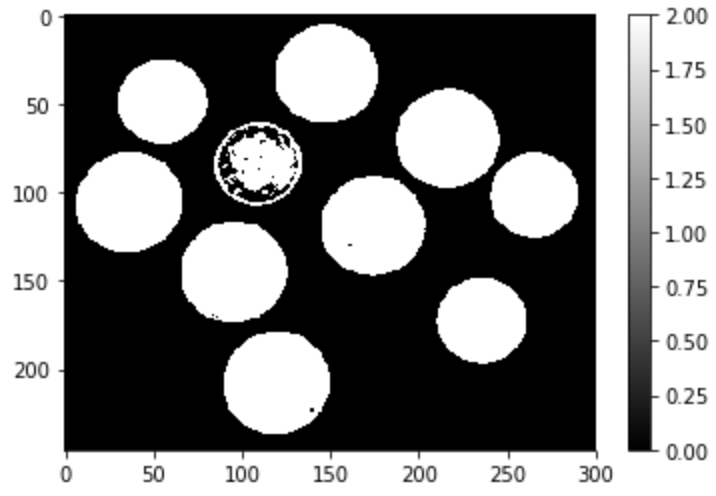
\includegraphics[width=\linewidth]{Materials/E4/coins_seg}
		\caption{Coins image segmented.}
	\end{subfigure}
	\hfill
	\begin{subfigure}[b]{0.45\linewidth}
		\centering
		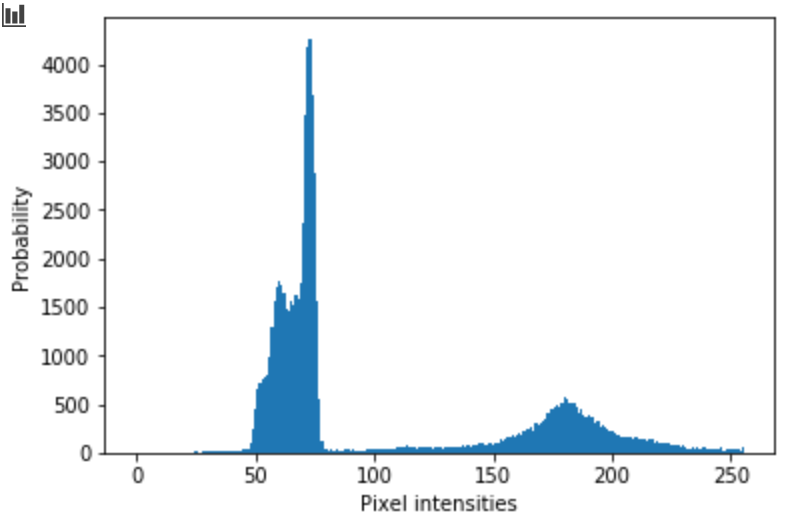
\includegraphics[width=\linewidth]{Materials/E4/coins_hist}
		\caption{Histogram of coins image.}
	\end{subfigure}
	\\
	\begin{subfigure}[b]{0.45\linewidth}
		\centering
		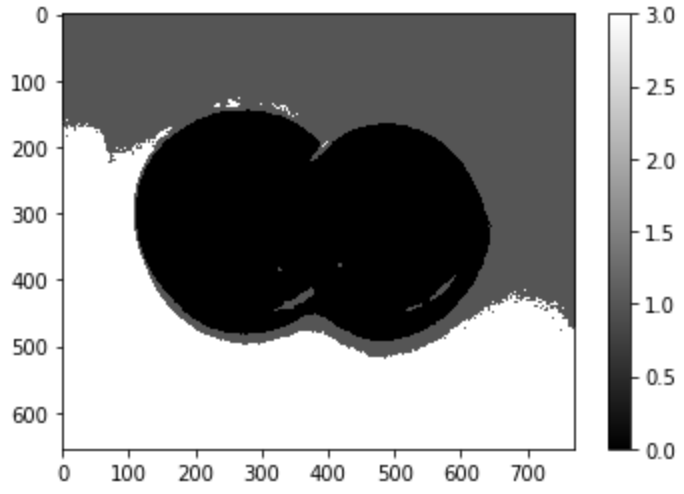
\includegraphics[width=\linewidth]{Materials/E4/euros_seg}
		\caption{Euros image segmented.}
	\end{subfigure}
	\hfill
	\begin{subfigure}[b]{0.45\linewidth}
		\centering
		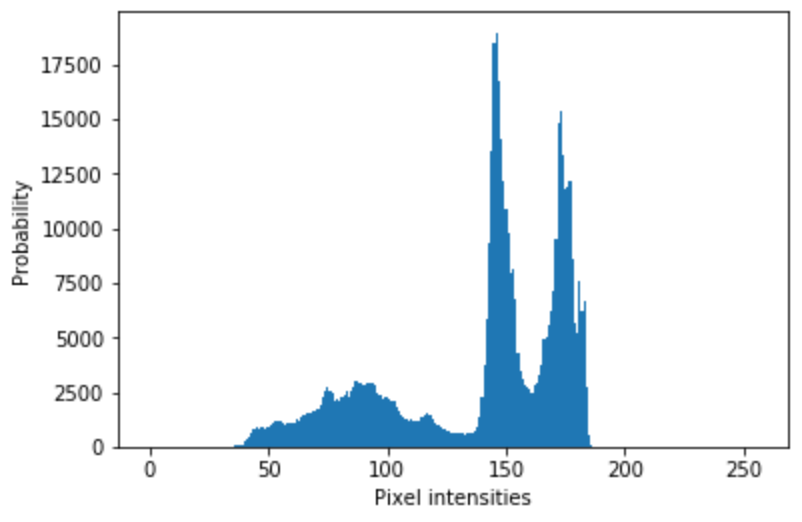
\includegraphics[width=\linewidth]{Materials/E4/euros_hist}
		\caption{Histogram of euros image.}
	\end{subfigure}
	\caption{Results of automated histogram segmentation.}
	\label{segmentations}
\end{figure}
In \autoref{segmentations} we see the results of automatically segmenting the coins and euros image. In \autoref{E4code} we see the code used for this exercise. To find the peaks in the histogram, we go through all intensity values and for each intensity we check the past 20 intensities, and the future 20 intensities and check if the amount of pixels with this intensity is the maximum over these intensities. This way we only get one peak despite the number of pixels close to each other in intensity fluctuates bit. We also check whether at least $0.05\%$ of the total amount of pixels have this intensity. Both the width we search with and the percentage of total pixels we want minimum are adjustable parameters, but I found these values worked well for our two test images.\\
Next we want to determine the thresholds. For this we want one threshold less than there are peaks, and we want these thresholds to be roughly in the middle between two peaks. For this reason, we in turn find the mean intensity between the current peak we are looking at and the next.  We search $\pm15$ intensities to find the intensity with least pixels to find the most natural break. When we no longer have a 'next' peak, we 'group' all pixel intensities above the last threshold we found. As we see in \autoref{segmentations} the histogram of the coins image has two peaks which the function finds and performs a good segmentation of the images. Only a few pixels in two of the coins has been misclassified and the very dark coin is as expected not segmented as well as the rest of the coins. In the euros histogram we see three peaks, one dark quite flat, and two high intensity peaks. The result is a segmentation of the two coins as one grouping, the lower part as one grouping and the upper part as the last grouping. The result is as expected as the upper part of the image is quite a bit darker then the lower part.\\
With this approach we can quite easily find a small to medium amount of peaks and segment these. We also get results which are as expected from a human perspective when we are looking at peaks in the histograms, that is, the function does not report a peak every time the histogram has a local maxima, but only when these local maxima are sufficiently spaced from each other. We can see this in both histograms in \autoref{segmentations} where from a human perspective we would only consider the left most part of the histogram of the coin image as one peak and not two. And the same for the right most part of the euros image (where we from a human perspective would consider 3 peaks, and not 4). However, the function has its limitations. If the peaks becomes too uniform, the function would have a hard time separating the real peaks and the 'false'-local-maxima-peaks. But also if we only have one peak the function would have issues. One peak could appear if we have a histogram with the shape of a very peaky normal distribution. Then we could imagine the left part of the image being black, gradually becoming grey, and then the right part of the image gradually becoming white. From a human perspective, this would need three groupings, but the function would segment the whole image as one grouping.\\
As we use the histogram to select the thresholds, and the only difference between a histogram of a low resolution image and a high resolution image is the numbers along the y-axis, the quality of the image has a low influence on the results of the segmentation. If we upped the resolution of the images we would get more total pixels, and perhaps more pixels where there already are a lot of pixels as the distribution of the histogram would remain unchanged. This means it perhaps would be easier to identify peaks, but as we already require a peak to consist of some percentage of the total pixels to be considered a peak, it would not have much influence.

\begin{figure}[H]
	\centering
	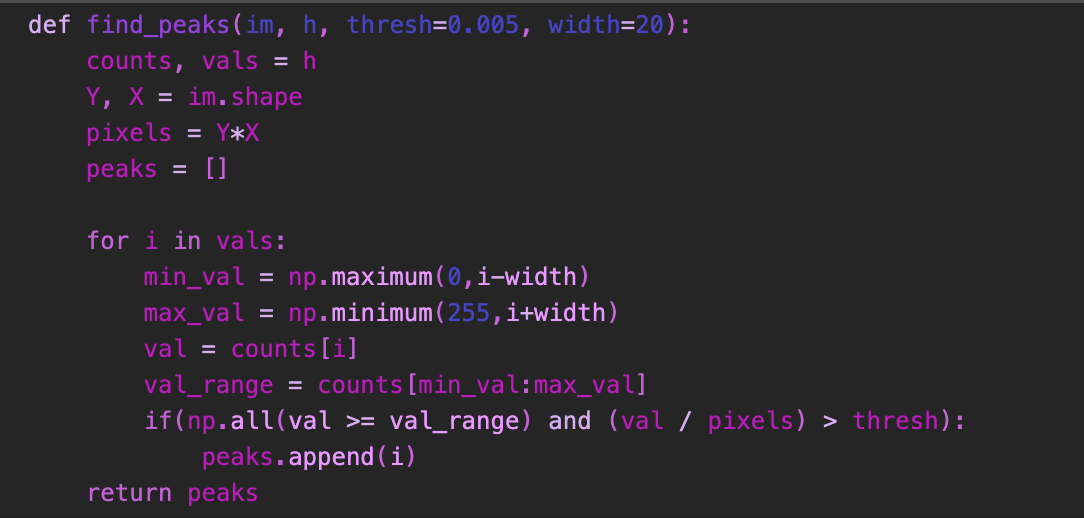
\includegraphics[width=0.8\linewidth]{Materials/E4/find_peaks}
	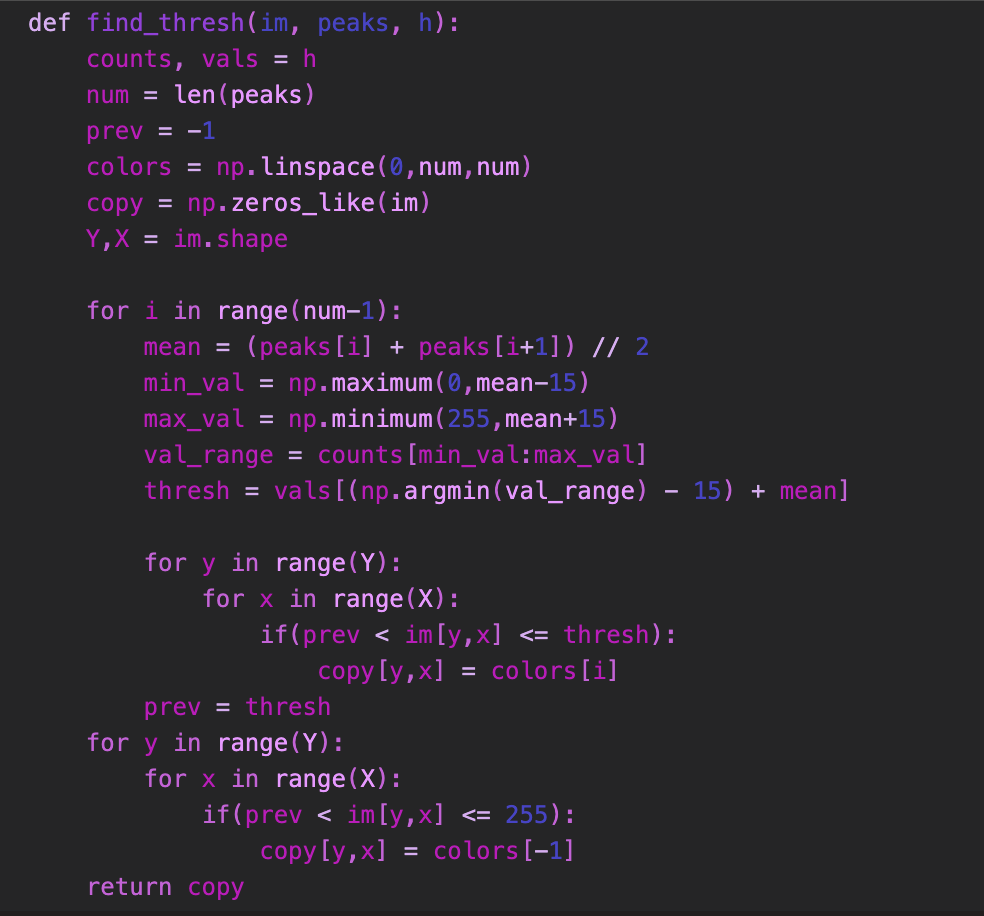
\includegraphics[width=0.8\linewidth]{Materials/E4/find_thresh}
	\caption{Code used for this exercise.}
	\label{E4code}
\end{figure}